\chapter{Personendetektion}
\label{chap:Personendetektion}

Auf der Grundlage der vorherigen Kapitel wird nun mittels einem neuronalen Netzwerk eine Personenerkennung erstellt. Dieser Abschnitt beschreibt das Vorgehen, um die Personenanzahl in einem Aufzug zu erkennen. In einem ersten Schritt wird die Verarbeitung der Rohdaten aufgezeigt. Für den Auswertealgorithmus wurden mehrere unterschiedliche Aufzüge evaluiert und für jeden Aufzug ein Profil erstellt. 


\section{Datenverarbeitung}

Mittels dem erstellten C-Programm ConvertValue\_V2 lassen sich die Rohdaten in \ac{CSV} Files konvertieren. Dabei wird über die USB-Schnittstelle mit dem Programm H-Term die \ac{ASCII}-Rohdaten ausgelesen. H-Term fügt zudem jedem Datensatz den aktuellen Zeitstempel an. In Abbildung \ref{fig:Dataframe} ist der Aufbau des Datenframes ersichtlich.

\begin{figure}[H]
	\centering
	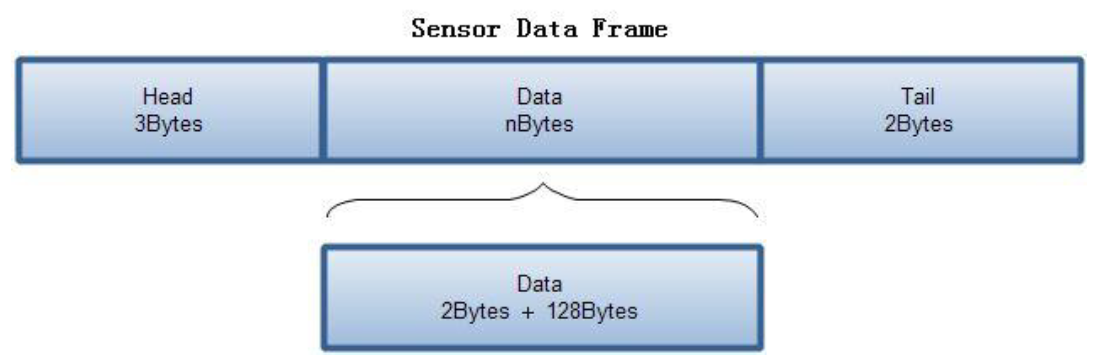
\includegraphics[width=0.5\textwidth]
	{fig/Dataframe}
	\caption[Datenframedes EVAL Boards]{Datenframe des Eval Boards}
	\label{fig:Dataframe}
\end{figure}

Der Header besteht aus der Zeichenfolge *** und wird zur Synchronisation benötigt. Danach folgen die 2 Byte für den Thermistorwert und 128 Byte für die Pixelwerte. Als Schluss wird die Zeile mit \textbackslash n \textbackslash r beendet.
Nachfolgend ist ein einzelnes Frame dargestellt:

17:34:04.009: \\
***\textcolor{blue}{‘r}h m l h f d \^ Z ` k f i g b Z Z X Z [ \_ a W X Y X Y V U T T U W U R R T U S U T X T R Q R R T V R R P S P U U V U Q P P O P Q V \textbackslash \textbackslash n \textbackslash r

Mit dem ConvertValue_V2 werden diese ac{ASCII}-Zeichen in die entsprechenden Fliesskommazahlen umgewandelt und formatiert. Nachfolgend ist die entsprechende Ausgabe ersichtlich.

26.000 ,27.250 ,27.000 ,26.000 ,25.500 ,25.000 ,23.500 ,22.500 ,24.000 ,26.750 ,25.500 ,26.250 ,25.750 ,24.500 ,22.500 ,22.500 ,22.000 ,22.500 ,22.750 ,23.750 ,24.250 ,21.750 ,22.000 ,22.250 ,22.000 ,22.250 ,21.500 ,21.250 ,21.000 ,21.000 ,21.250 ,21.750 ,21.250 ,20.500 ,20.500 ,21.000 ,21.250 ,20.750 ,21.250 ,21.000 ,22.000 ,21.000 ,20.500 ,20.250 ,20.500 ,20.500 ,21.000 ,21.500 ,20.500 ,20.500 ,20.000 ,20.750 ,20.000 ,21.250 ,21.250 ,21.500 ,21.250 ,20.250 ,20.000 ,20.000 ,19.750 ,20.000 ,20.250 ,21.500 ,\textcolor{blue}{25.0625} ,17:34:04.009

Sporadisch enstanden bei der Messung durch das Programm H-Term fehlerhafte Datensätze, da der mitgesendete Zeitstempel erst nach dem Header eingefügt wurde. Diese Fehler mussten von Hand korrigiert werden. 




\section{Datenmanipulation mittels Interpolation}

Die Auflösung von 8x8 Pixel bietet nur begrenzte Aussagekraft über die Anzahl Personen in einem Aufzug. Daher wurde mittels MATLAB mehrere Interpolationsverfahren benutzt, um die Auflösung der Wärmebildinformationen zu vergössern. Im Zusammenhang mit den Pixelwerten eignen sich die bikubische die lanczossche Interpolationsverfahren. Durch das lanczossche Interpolationsverfahren werden wärmere Gebiete stärker vom kühleren Hintergrund getrennt. Bei einer Interpolation von 8x8 Pixel auf 32x32 Pixel nähern sich beide Verfahren sehr stark an. 

Mit dem Ansatz, dass der interne Thermistor und der Hintergrund im Bildbereich der Umgebungstemperatur entspricht, lässt sich eine Korrektur durchführen. Werden alle Werte unterhalb der Umgebungstemperatur den Werten 0 und alle Werte oberhalb der Umgebungstemperatur dem Wert 1 zugeordnet, kann ein binäres Wärmebild generiert werden. Es lässt sich daraus die 

Dieser Ansatz bedingt jedoch, dass die Personen zu jeder Zeit höhere Temperaturen besitzten, als die Umgebungstemperatur.

In Hinsicht auf das neuronale Netzwerk bieten vor allem grössere Auflösungen mehr Spielraum für das Convolution Neural Network. Die Auflösung ist entscheidend, da 



\begin{figure}[!ht]
	\centering
	\begin{minipage}[c]{0.3\linewidth}
	\centering
	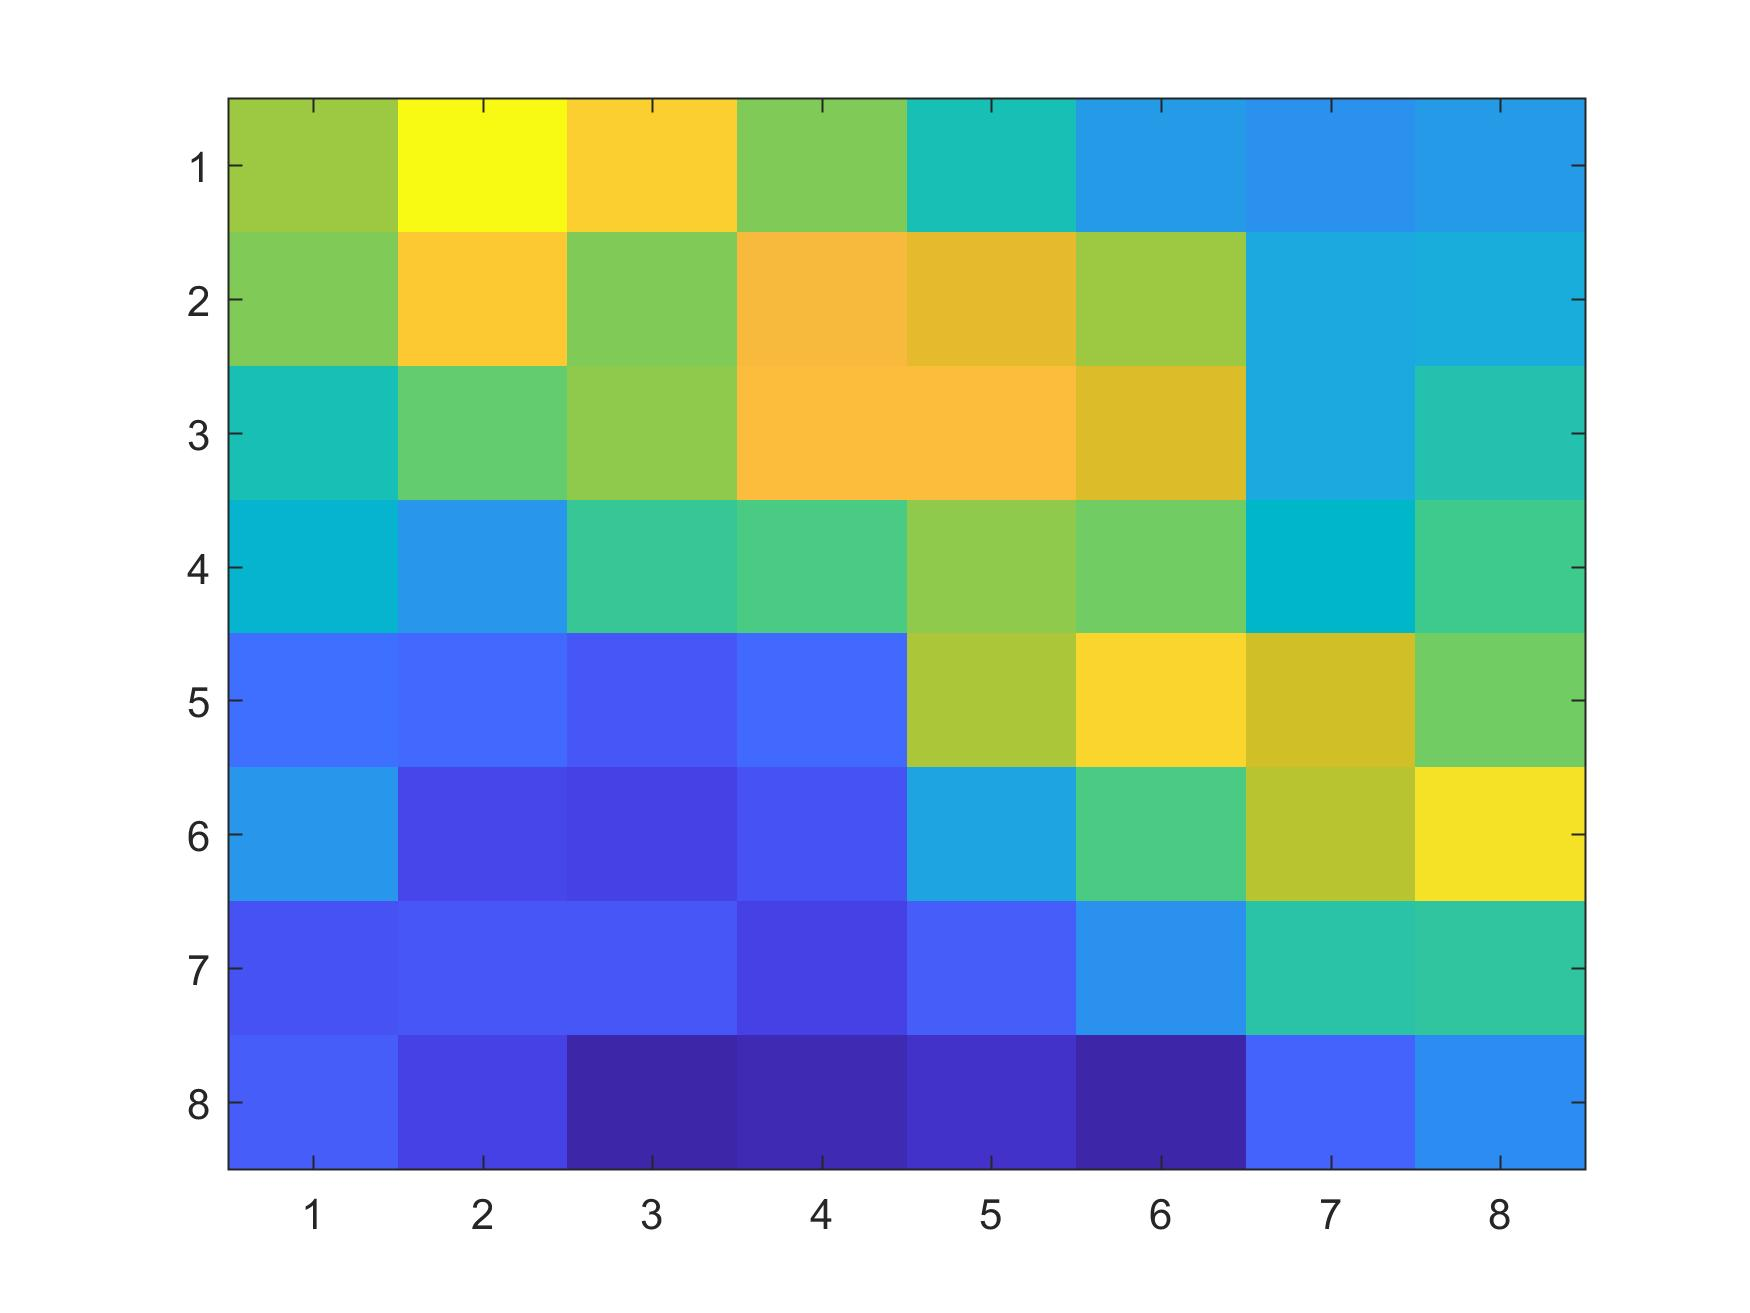
\includegraphics[width=1.0\linewidth]{fig/interpol_1}
	\caption[Originalframe]{Originalframe}
	\label{fig:interpol2}
	\end{minipage}
	\begin{minipage}[c]{0.3\linewidth}
		\centering
	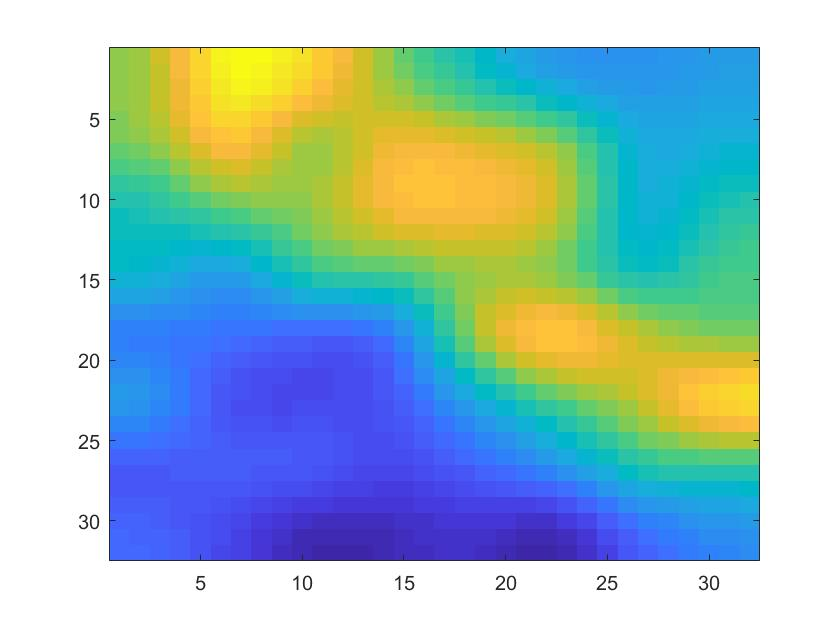
\includegraphics[width=1.0\linewidth]{fig/interpol_2}
	\caption[bikubische interpoliert]{Interpolation}
	\label{fig:interpol2}
	\end{minipage}
	\begin{minipage}[c]{0.3\linewidth  }
			\centering
	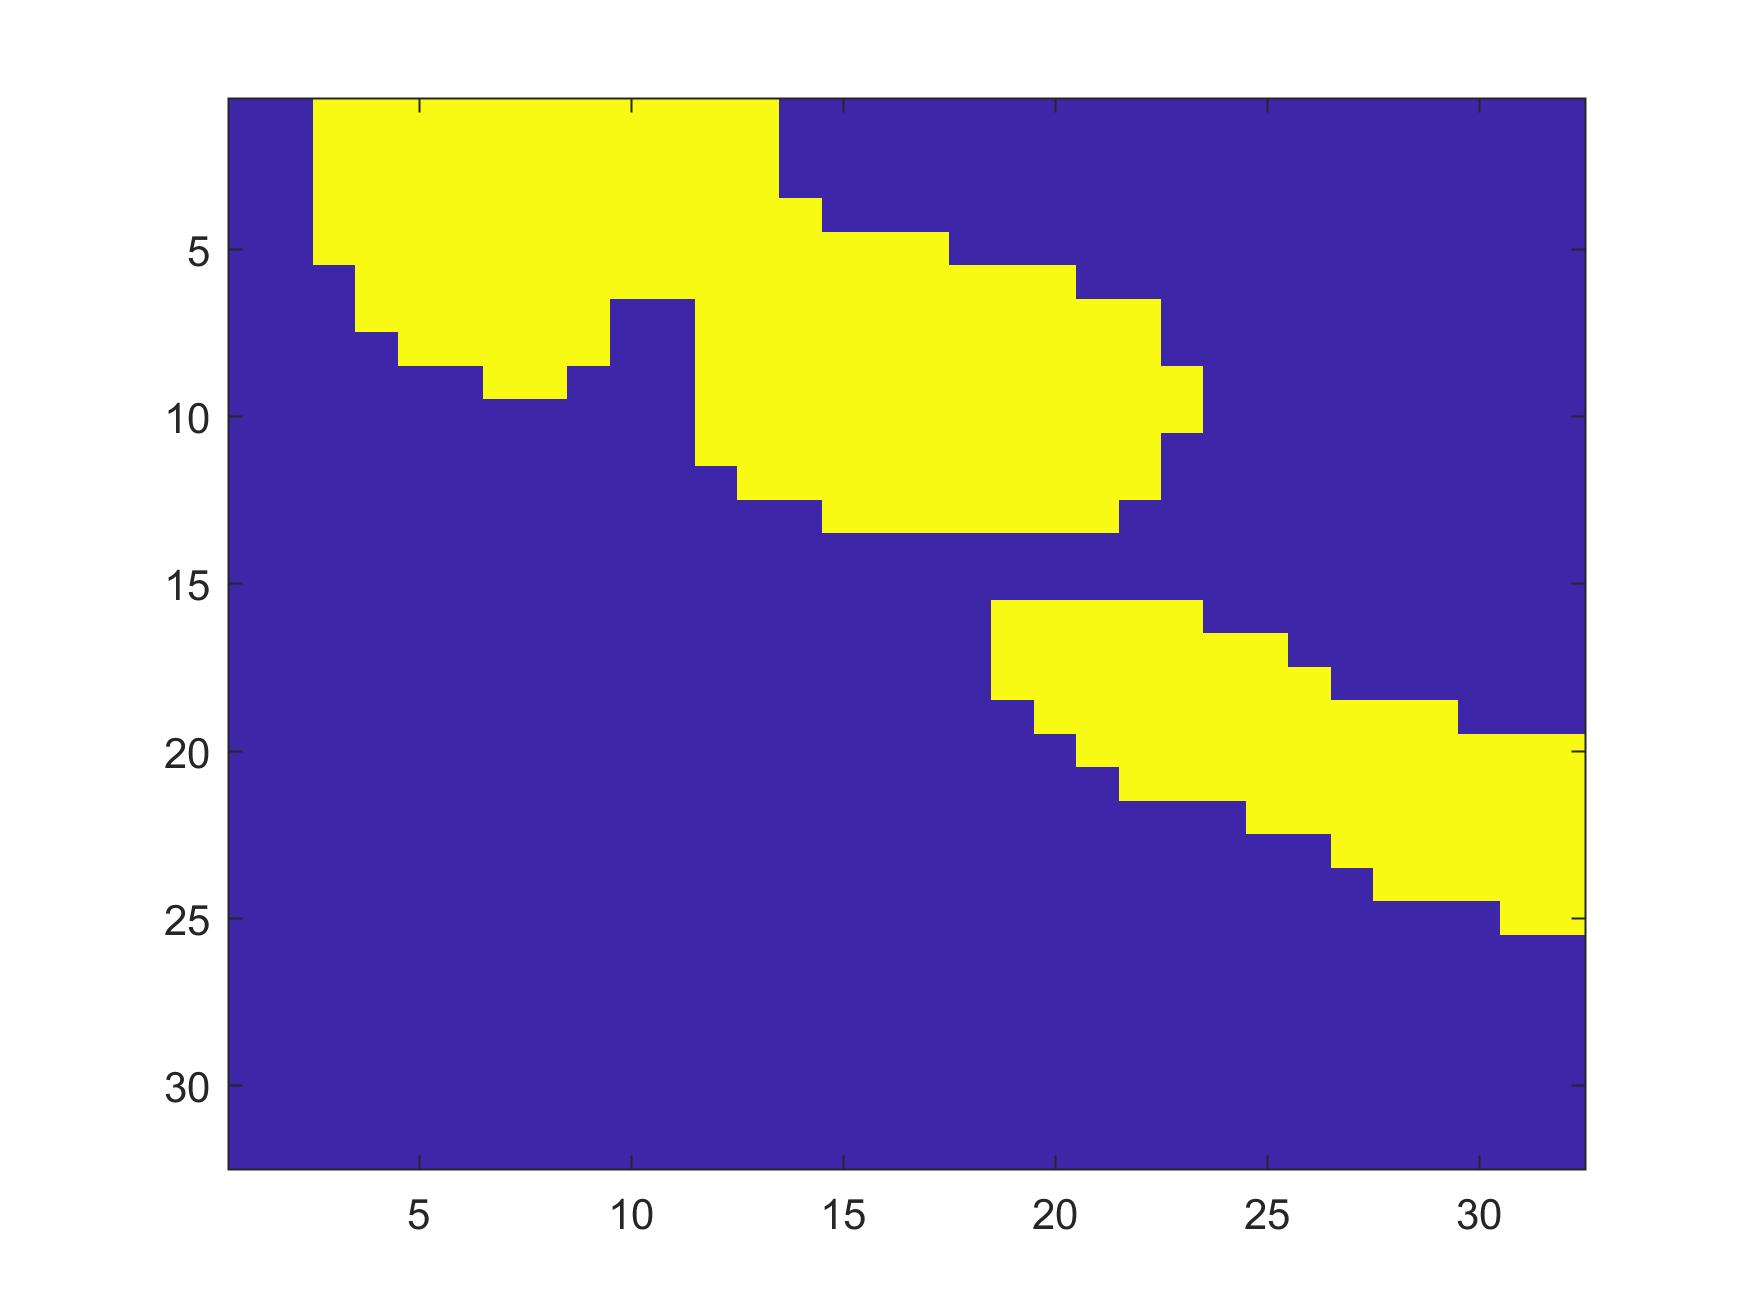
\includegraphics[width=1.0\linewidth]{fig/interpol_3}
	\caption[Temperaturkorrektur]{Temperaturkorrektur}
	\label{fig:interpol3}
\end{minipage}
\end{figure}


Nachteilig ist bei der Interpolation, das die Wärmebildinformationen mit zunehmender Grösse zum Teil stark verfälscht werden. Da sich die Zwischenräume nur rechnerisch bilden lassen. Es wurde daher entschieden, die Auflösung bei den unverfäschten, originalen Frames zu belassen. Da so keine Bildinformationen manipuliert werden oder verloren gehen. 



\section{Symmetrische Erweiterung}

Um die Datensätze zu vergrößern wurden die drei Profile erweitert. Dafür wurde für die entsprechenden Profile Python-Programm rotate\_and\_swap\_ProfilX  geschrieben, welche alle Frames er Datensätze symmetrisch erweitert.  

\begin{figure}[!ht]
	\centering
	\begin{minipage}[c]{0.35\linewidth}
	\centering
	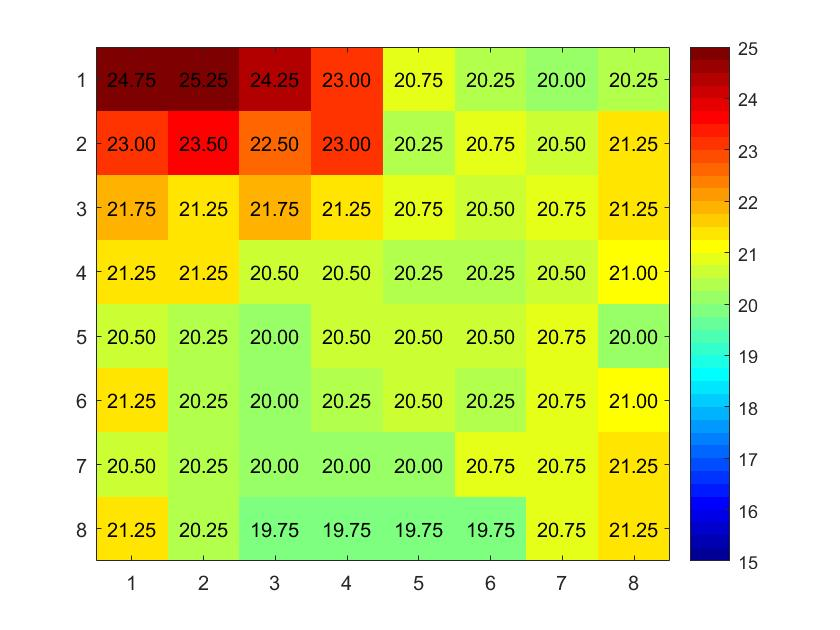
\includegraphics[width=.8\linewidth]{fig/original}
	\caption{Originales Frame}
	\label{fig:original}
	\end{minipage}
	\hfill
	\begin{minipage}[c]{0.6\linewidth  }
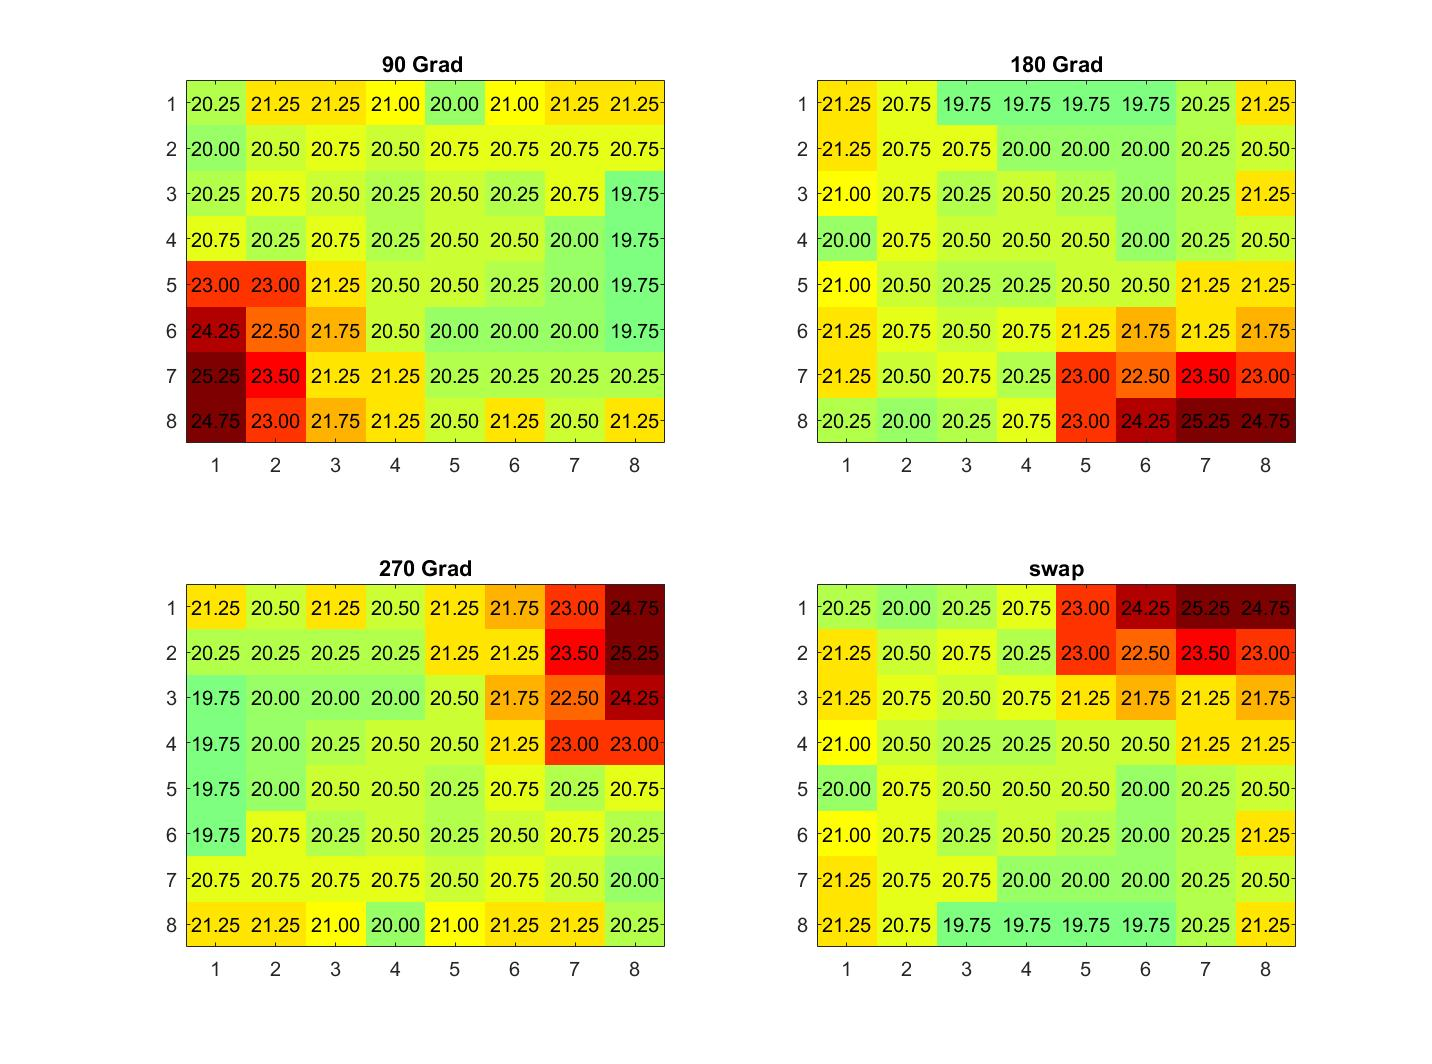
\includegraphics[width=1\linewidth]{fig/rotated}
\caption{Rotierte und gespiegelte Frames}
\label{fig:rotated}
	\end{minipage}
\end{figure}


Durch die Erweiterung konnten die Datensätze um den Faktor 5 vergrößert werden. Es konnten so, nicht vermessenen Positionen generiert werden. Mit den Messstandorten A-I und den generierten Erweiterungen werden nahezu beliebige Varianten im Messbereich zur Verfügung.


\subsection{Profilbildung}

In den entsprechenden rawdatamerge werdend ie daten zu einem 



Profil 1
Size of:
- Training-set:         126936
- Validation-set:       25000

Profil 2



Profil 3


Testprofil Test-set:             22169




\section{Aufbau Convolution Neural Network}




Convolutional Networks work by moving small filters across the input image. This means the filters are re-used for recognizing patterns throughout the entire input image. This makes the Convolutional Networks much more powerful than Fully-Connected networks with the same number of variables. This in turn makes the Convolutional Networks faster to train




The convolutional filters are initially chosen at random, so the classification is done randomly. The error between the predicted and true class of the input image is measured as the so-called cross-entropy. The optimizer then automatically propagates this error back through the Convolutional Network using the chain-rule of differentiation and updates the filter-weights so as to improve the classification error. This is done iteratively thousands of times until the classification error is sufficiently low.


(W -F +2P) : S+ 1



\begin{figure}[H]
	\centering
	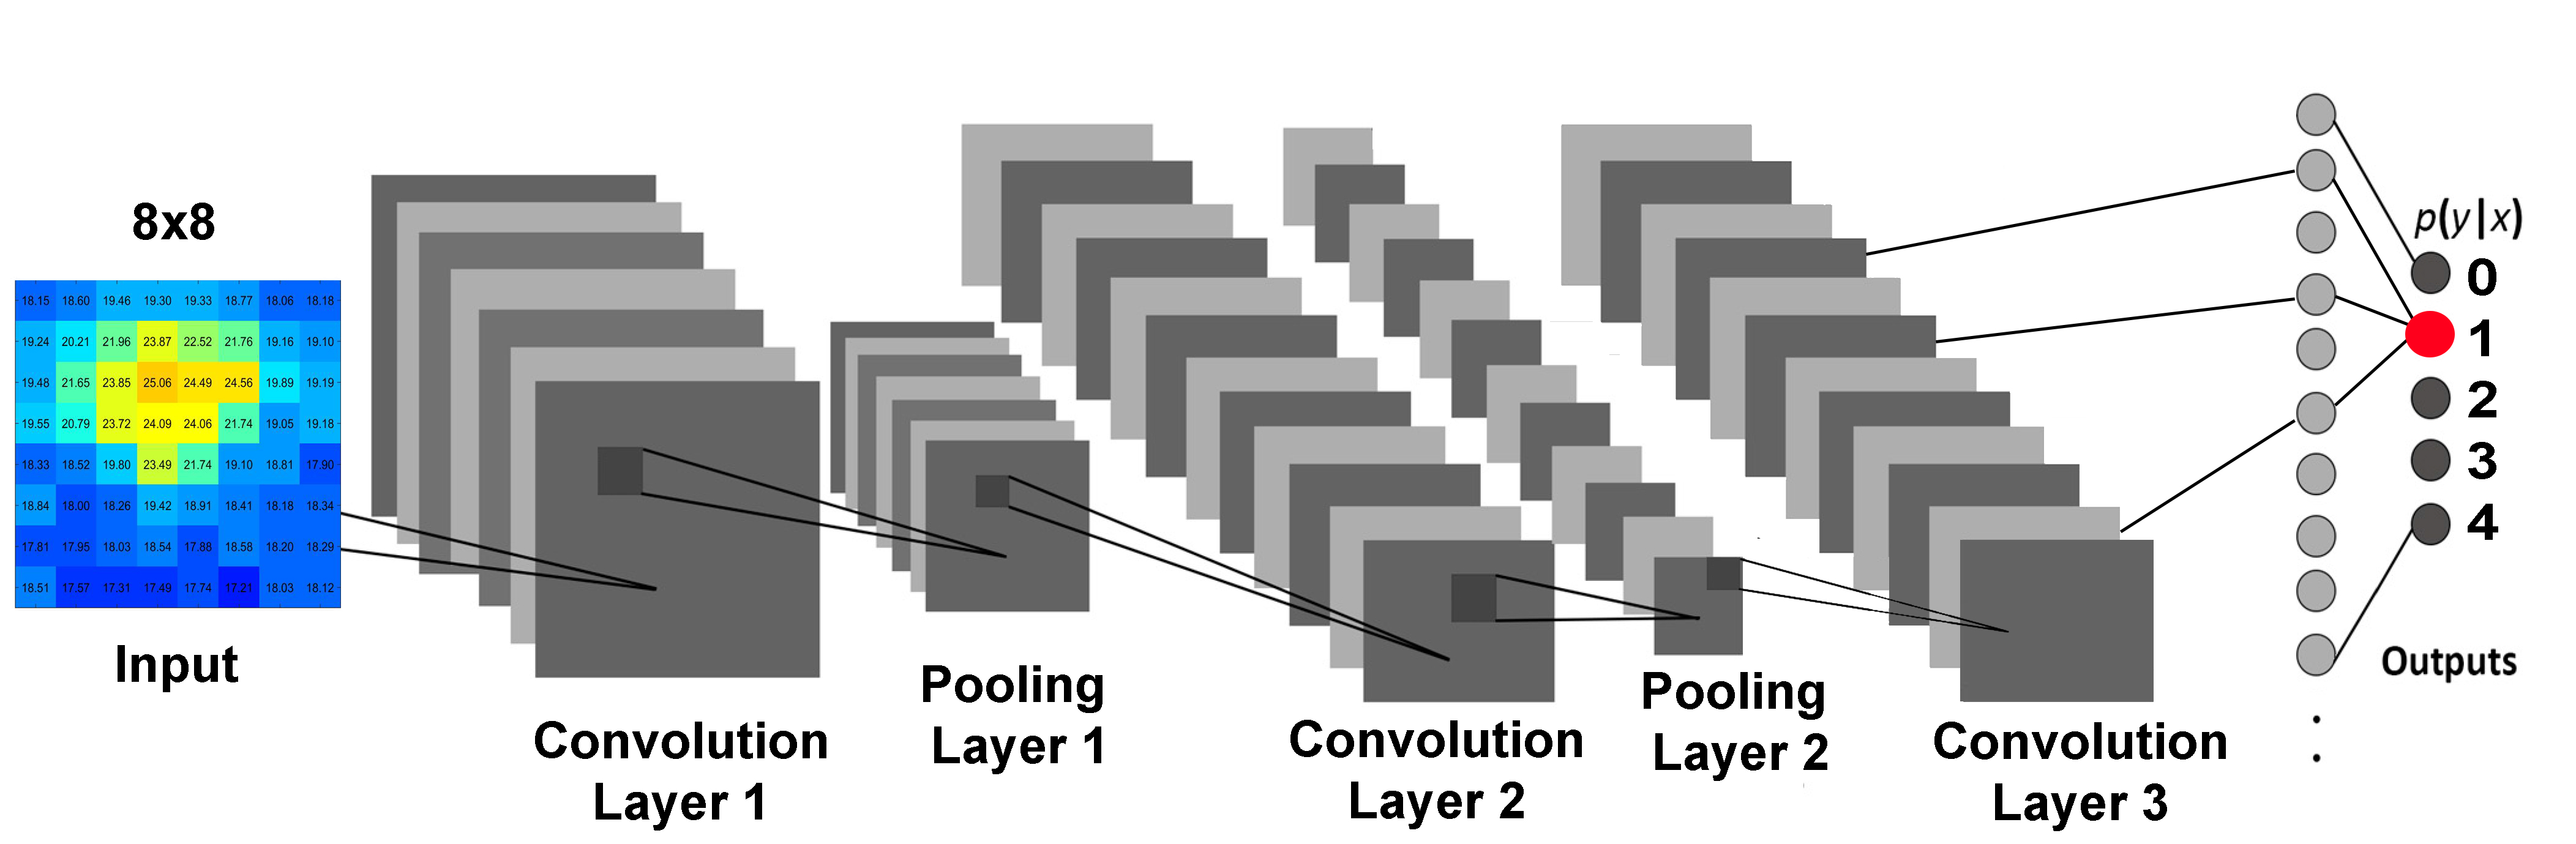
\includegraphics[width=1\textwidth]
	{fig/CNN_broschuere.jpg}
	\caption[Aufbau des Convolutional Neural Network]{Aufbau des Convolutional Neural Network}
	\label{fig:CCN}
\end{figure}




\section{Training und Validierung}




\begin{figure}[H]
	\centering
	\caption{Trainingsverlauf Profil 1}
	\label{fig:traininsverlauf}
	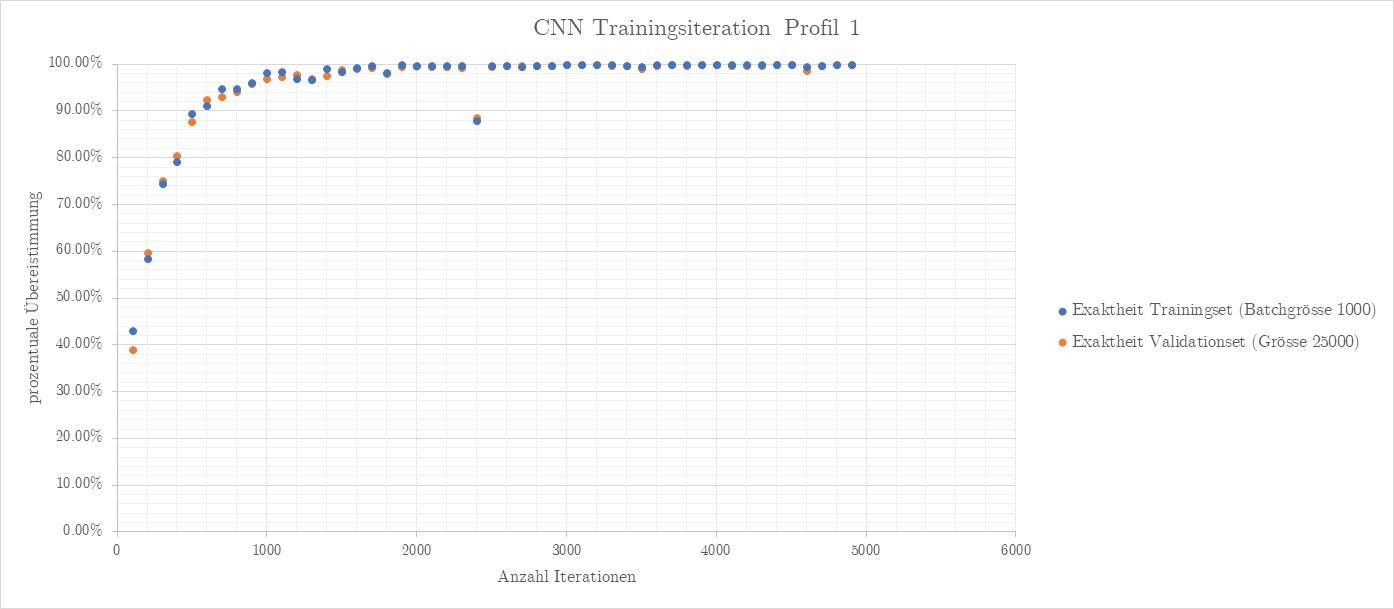
\includegraphics[width=1.0\linewidth]{fig/Traininsverlauf}
\end{figure}


\section{Ergebnisse}


\subsection{Profil 1}

\begin{figure}[H]
	\centering
	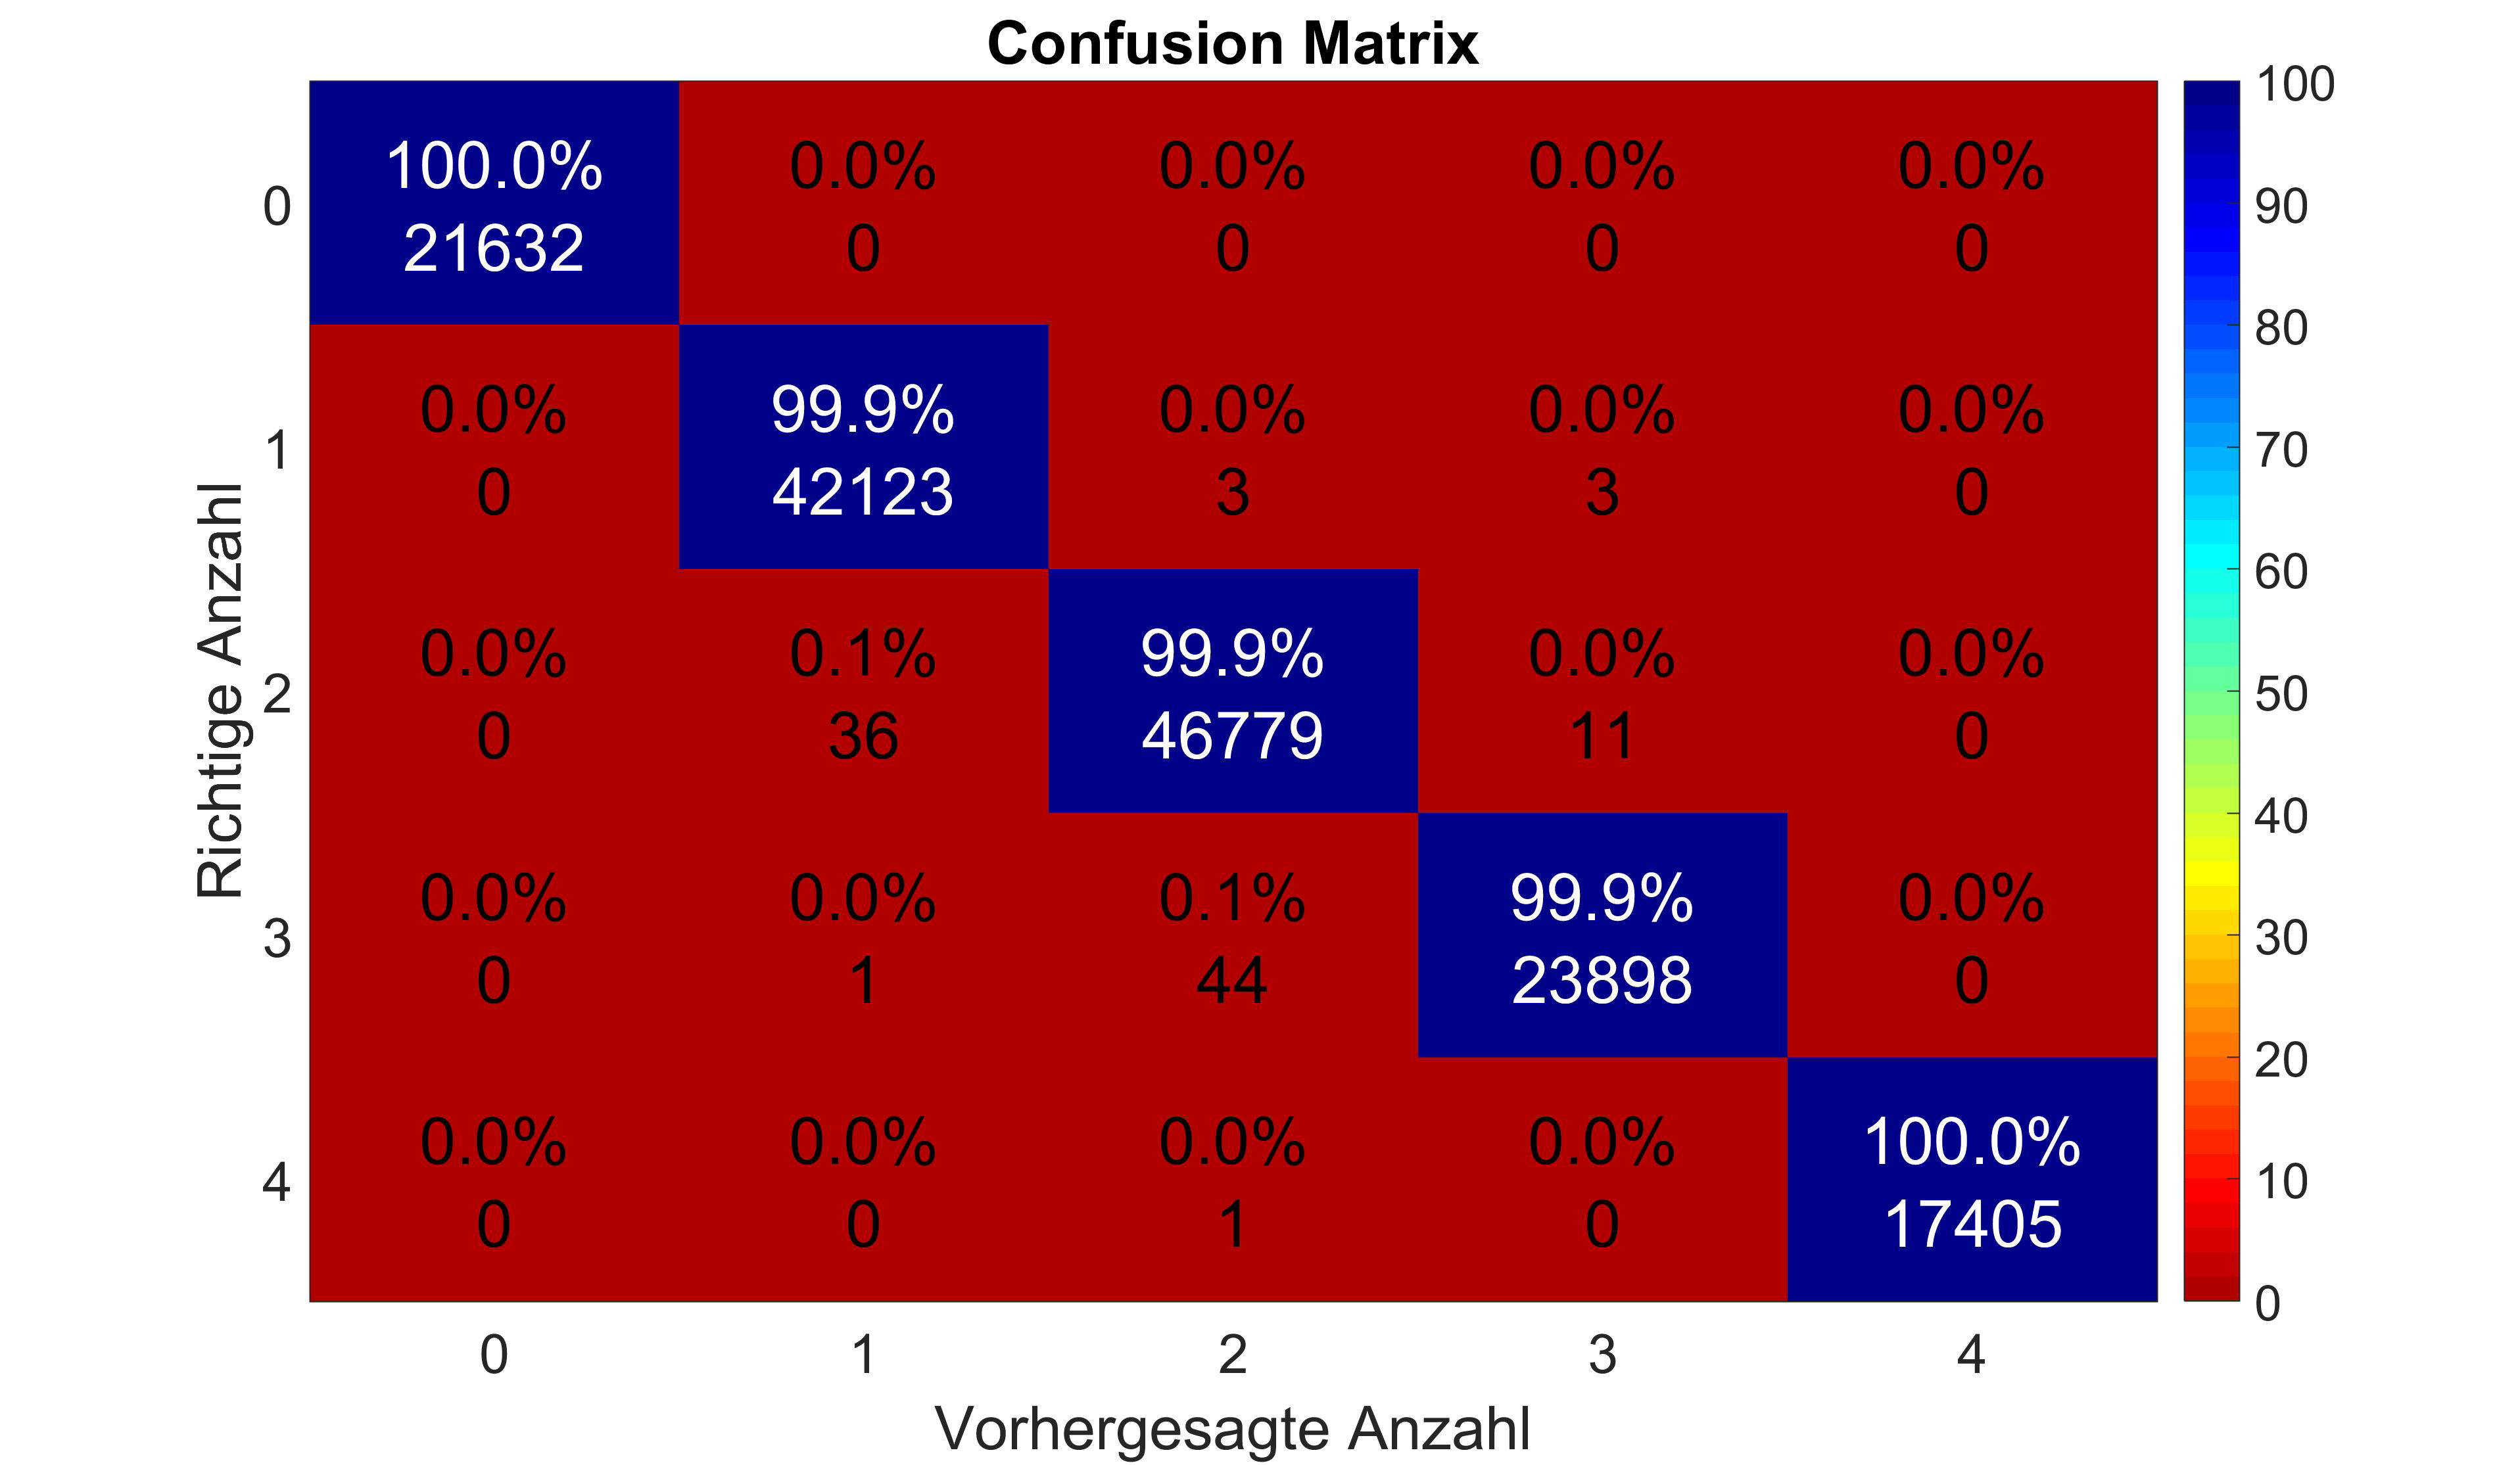
\includegraphics[width=0.7\linewidth]{fig/Profil_1}
	\caption{Confusion Matrix Profil 1}
	\label{fig:profil1}
\end{figure}

\subsection{Profil 2}

\begin{figure}[H]
	\centering
	\includegraphics[width=0.7\linewidth]{fig/Profil_2}
	\caption{Confusion Matrix Profil 2}
	\label{fig:profil2}
\end{figure}



\subsection{Profil 3}

\begin{figure}[H]
	\centering
	\includegraphics[width=0.7\linewidth]{fig/Profil_3}
		\caption{Confusion Matrix Profil 3}
	\label{fig:profil3}
\end{figure}

\section{Echtzeitpersonenerkennung}

Dank der Saver-Klasse von Tensorflow lassen sich erstellte \ac{CNN}-Modell als ckpt-File speichern. Dabei werden alle trainierten Bias und Gewichtungen in ein ckpt-File gespeichert. Diese lassen sich wiederum in ein untrainiertes CNN laden.

Auf dieser Grundlage wurde eine Messeinheit erstellt, welche mittels trainiertenn CNN zur Echtzeit Personerkennungen durchführt. Die Messeinheit besteht aus einenm AMG8834 Eval Kit, einem Raspbery Pi3 und einer Powerbank.

In Abbildung ist das 


\begin{figure}[H]
	\centering
	\label{fig:Echtzeitmesseinheit}
	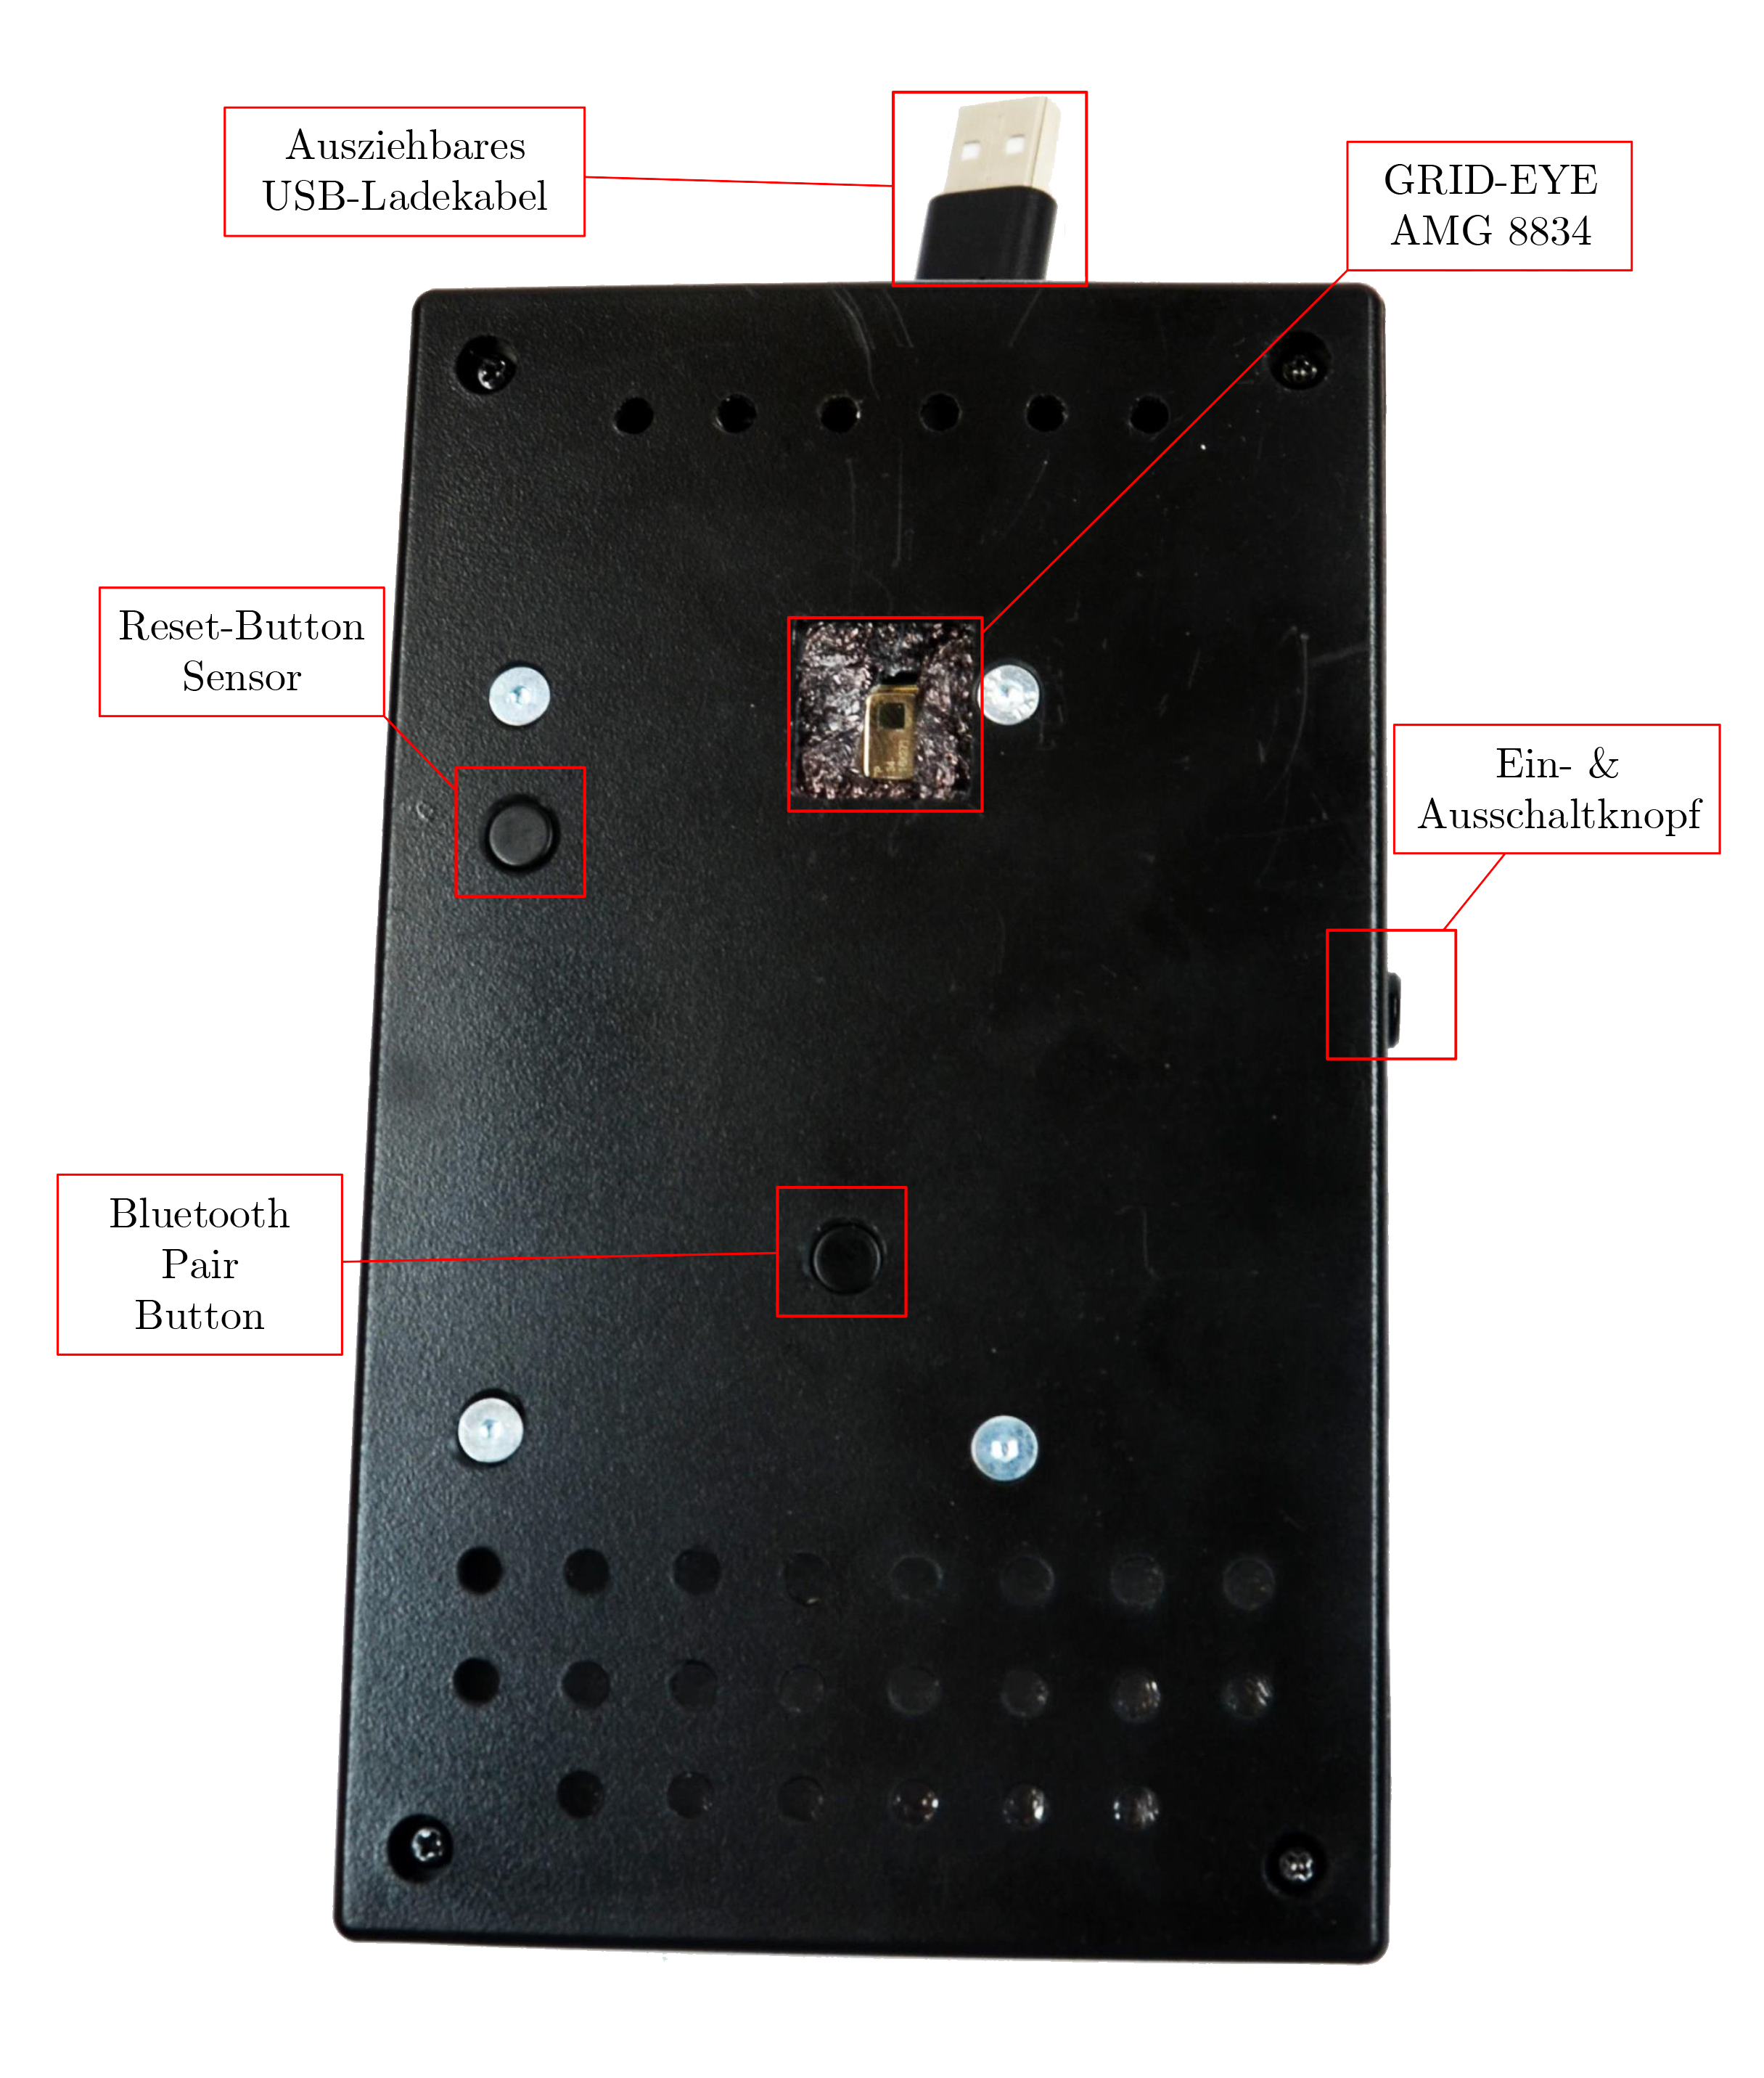
\includegraphics[width=0.8\linewidth]{fig/Echtzeitmessgeraet.jpg}
		\caption{Trainingsverlauf Profil 1}
\end{figure}




\section{Fazit}

Tensorflow bietet mit der Implentierung eines \ac{CNN} eine grosse Anzahl an Parameter und varrierbaren Einstellungen, um eine Bilderkennung mittels maschinellen Lernens zu realiiseren. 

Der relevanteste Punkt für die Personenerkennung sind die Trainingssets. Es wurde mit den erstellten Datensätzen eine möglichst breite Platte an Situationen generiert, trotzdem lassen sich zum Teil Frames nicht differenzieren. Dies hat eines der folgenden Gründe.

Die Auflösung ist jedoch in diesem Zusammenhang. Da nur 8x8 Pixel zur Verfügung stehen, ist die Tiefe de neuronalen Netzwerk begrenzt. Es lassen sich viele Features aus den Frames generieren , doch die Unterschiede zu anderen Objekten lassen sich nur bedingt erstellen.

Die Genauigkeit des Sensors streut mit 3°C bedeutend. Dies verursacht das die bedeutend mehr unterschiedliche thermische Frames vorhanden sind, doch die Streuung verursacht eine grösse Messunsicherheit, welche vorallem bei Bilder zu tragen kommen, in welchen mehrere Personen von unterschieldicher Grösse nahe beinader stehen. Durch die Unsicherheit lassen sich einzelne grosse Personen kaum von mehreren kleinen Personen differenzieren.






